\documentclass[aspectratio=43]{beamer}
\usepackage[utf8]{inputenc}
\usepackage[T1]{fontenc}
\usepackage{listings}

\graphicspath{{img/}{build/}{./}}

\title[Autonomous Calibration]{\large {Autonomous Calibration}\\ of 3D Computer Vision System}
\date{WASP Positioning Sales Pitch}
% \author[Gustaf]{Gustaf Waldemarson \texttt{gustaf.waldemarson@arm.com}}

\usetheme{WASP}

\lstloadlanguages{[ISO]C++}
\lstdefinestyle{google-c++}{%
  language = {[ISO]C++},
  captionpos = {t},
  frame = {lines},
  columns = {fixed},
  numbers = {left},
  numberstyle = {\tiny},
  numbersep = {5pt},
  breaklines = {true},
  basicstyle = {\footnotesize},
  identifierstyle = {\ttfamily},
  keywordstyle = {\color[rgb]{0, 0, 1}},
  commentstyle = {\color[rgb]{0.026,0.112,0.095}},
  stringstyle = {\color[rgb]{0.627,0.126,0.941}},
  numberstyle = {\color[rgb]{0.205, 0.142, 0.73}},
  backgroundcolor = {\color[rgb]{0.9, 0.9, 0.9}},
}


\begin{document}

\begin{frame}
  \titlepage
\end{frame}

\begin{frame}{The Correspondence Problem}

  \begin{figure}
    \centering
    \includegraphics[width=0.5\textwidth]{img/correspond}
  \end{figure}

  \begin{itemize}
  \item One of the major problem in computer vision is finding image points that
    correspond to the same 3D point in a scene. In the field, this is known as the
    correspondence problem.
  \item There is no easy solution -- The best we can do is use heuristic to find
    points that are likely to correspond.
  \end{itemize}
\end{frame}


\begin{frame}{Off-the-shelf Algorithms}

  For the vision aspect of this project, the aim was to use primarily
  off-the-shelf algorithms to solve our problem.

  \begin{itemize}
  \item To This end, \emph{OpenCV} was used to perform the heavy lifting in
    regard to image detection and matching,
  \item and the \emph{Ceres Solver} was used to run large scale non-linear
    optimizations based on our problem formulations.
  \end{itemize}

  \begin{figure}
    \centering
    
\includegraphics[width=0.2\textwidth]{img/opencv}
  \end{figure}

\end{frame}


\begin{frame}{Inferring 3D Structure}
  \begin{itemize}
  \item In order to properly find the intrinsic parameters of the camera, we
    need to infer some 3D structure from the environment. To that end, we need
    to do the following:
    \begin{itemize}
    \item Find keypoints via \emph{Feature Detection}.
    \item Match these keypoints through \emph{Feature Matching}.
    \item Summarize the matches into \emph{Tracks}.
    \item Find camera parameters and 3D points through \emph{Optimization}.
    \end{itemize}
  \item Each of these steps will be described in more details.
  \end{itemize}
\end{frame}


\begin{frame}{Feature Detection}

  \begin{itemize}
  \item The first thing that must be done is finding image points, or keypoints,
    that are likely to be seen across multiple images.
  \item While \emph{SIFT} is the most well known keypoint detector, it has some
    limitations and is also a patented algorithm, meaning it cannot be used
    commercially without paying licensing fees.
  \item To this end, we opted to use the \emph{ORB} feature points; which is
    claims to be both better and faster than \emph{SIFT}.
  \end{itemize}

  \begin{figure}
    \centering
    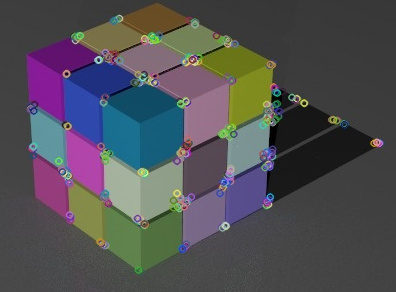
\includegraphics[width=0.38\textwidth]{img/kps_0}
  \end{figure}

\end{frame}



\begin{frame}{Feature Matching}

  Once keypoints have been found in all images, they need to be matched across
  each other. To this end, we try to match keypoints in the following way:

  \begin{itemize}
  \item From each pair of images:
    \begin{itemize}
    \item Match keypoints using the descriptor based on the shortest hamming
      distance.
    \item From all of the matched keypoints, use RANSAC to compute the
      Fundamental Matrix ($F$) and use it to filter out as many outliers as
      possible.
    \end{itemize}
  \end{itemize}

  \begin{figure}
    \centering
    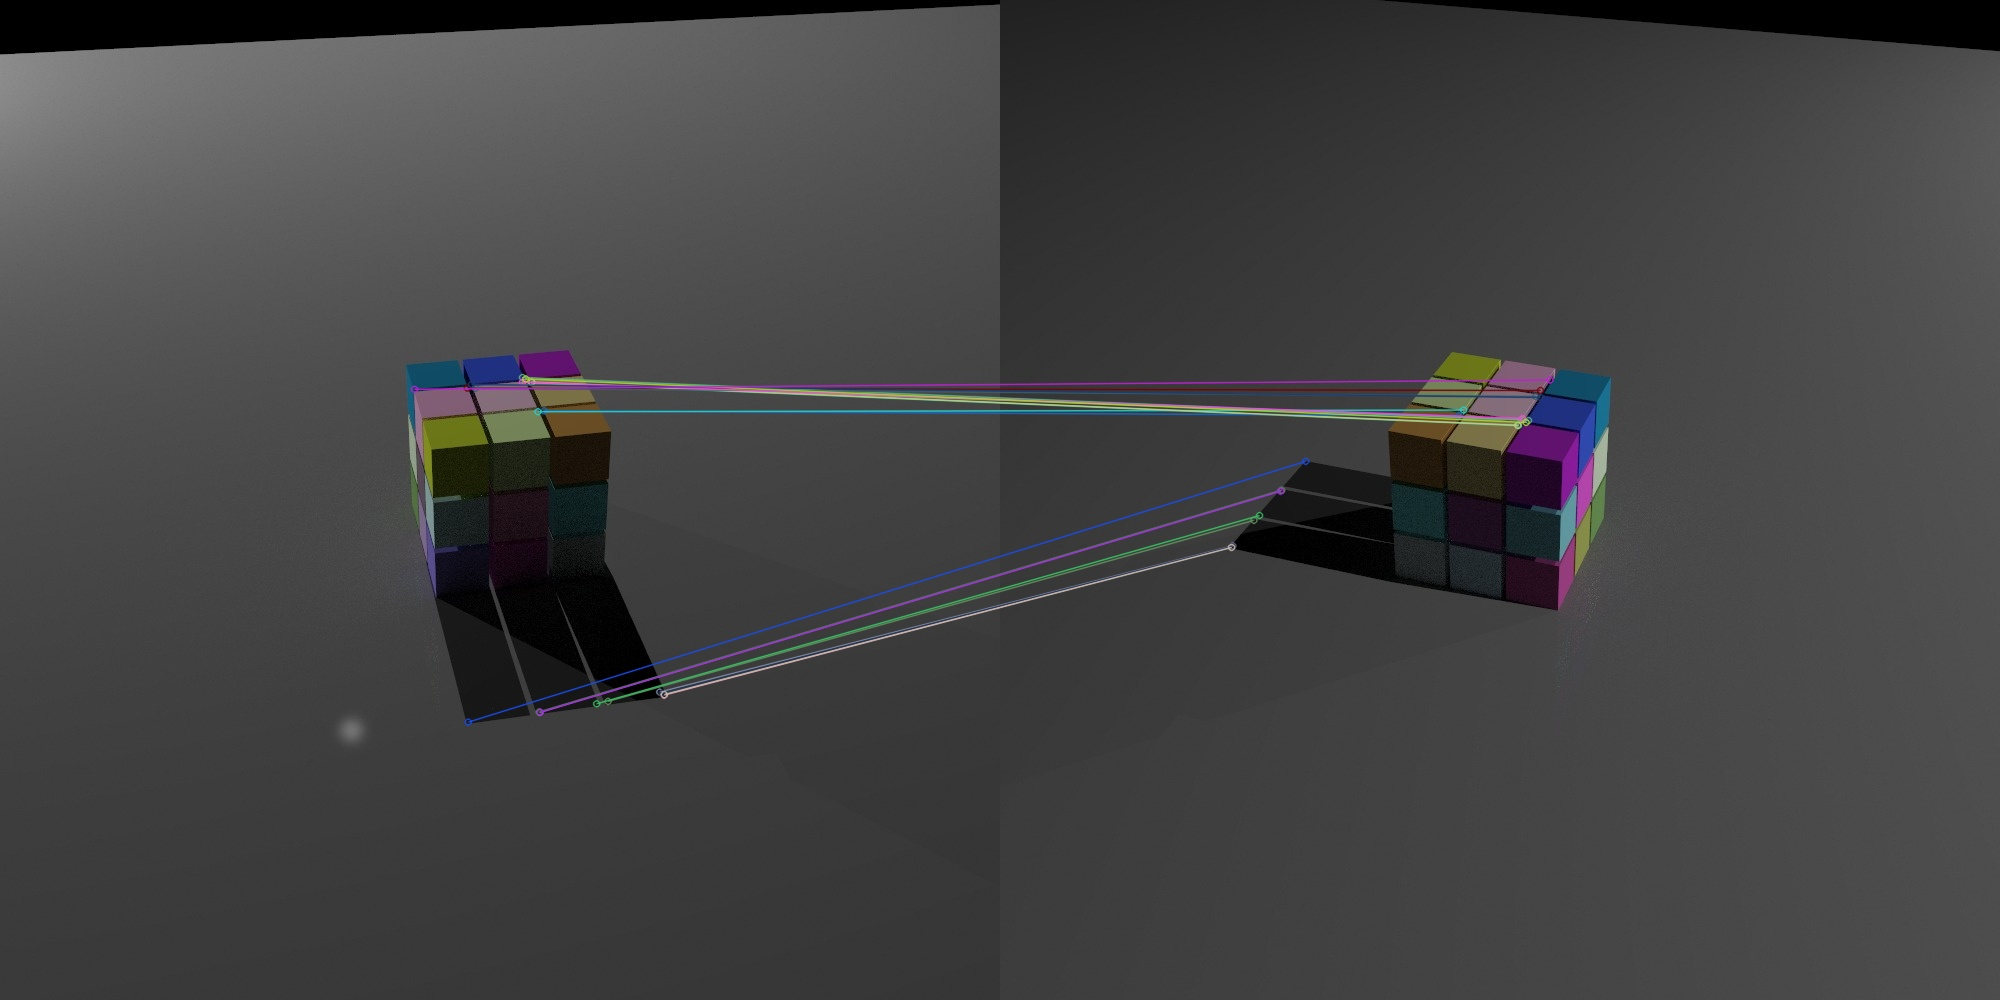
\includegraphics[width=0.42\textwidth]{img/matches_F_ransac_3}
  \end{figure}

\end{frame}


\begin{frame}{Track Detection}

  \begin{itemize}
  \item Finally, summarize all matches into a single graph, here dubbed the
    \emph{Image Graph}.
  \item Using some additional graph filtering techniques, some additional matches
    that are unlikely to be correct are removed.
  \item Finally, \emph{tracks} between multiple keypoints spanning multiple images
    are identified.
  \end{itemize}

  \begin{figure}
    \centering
    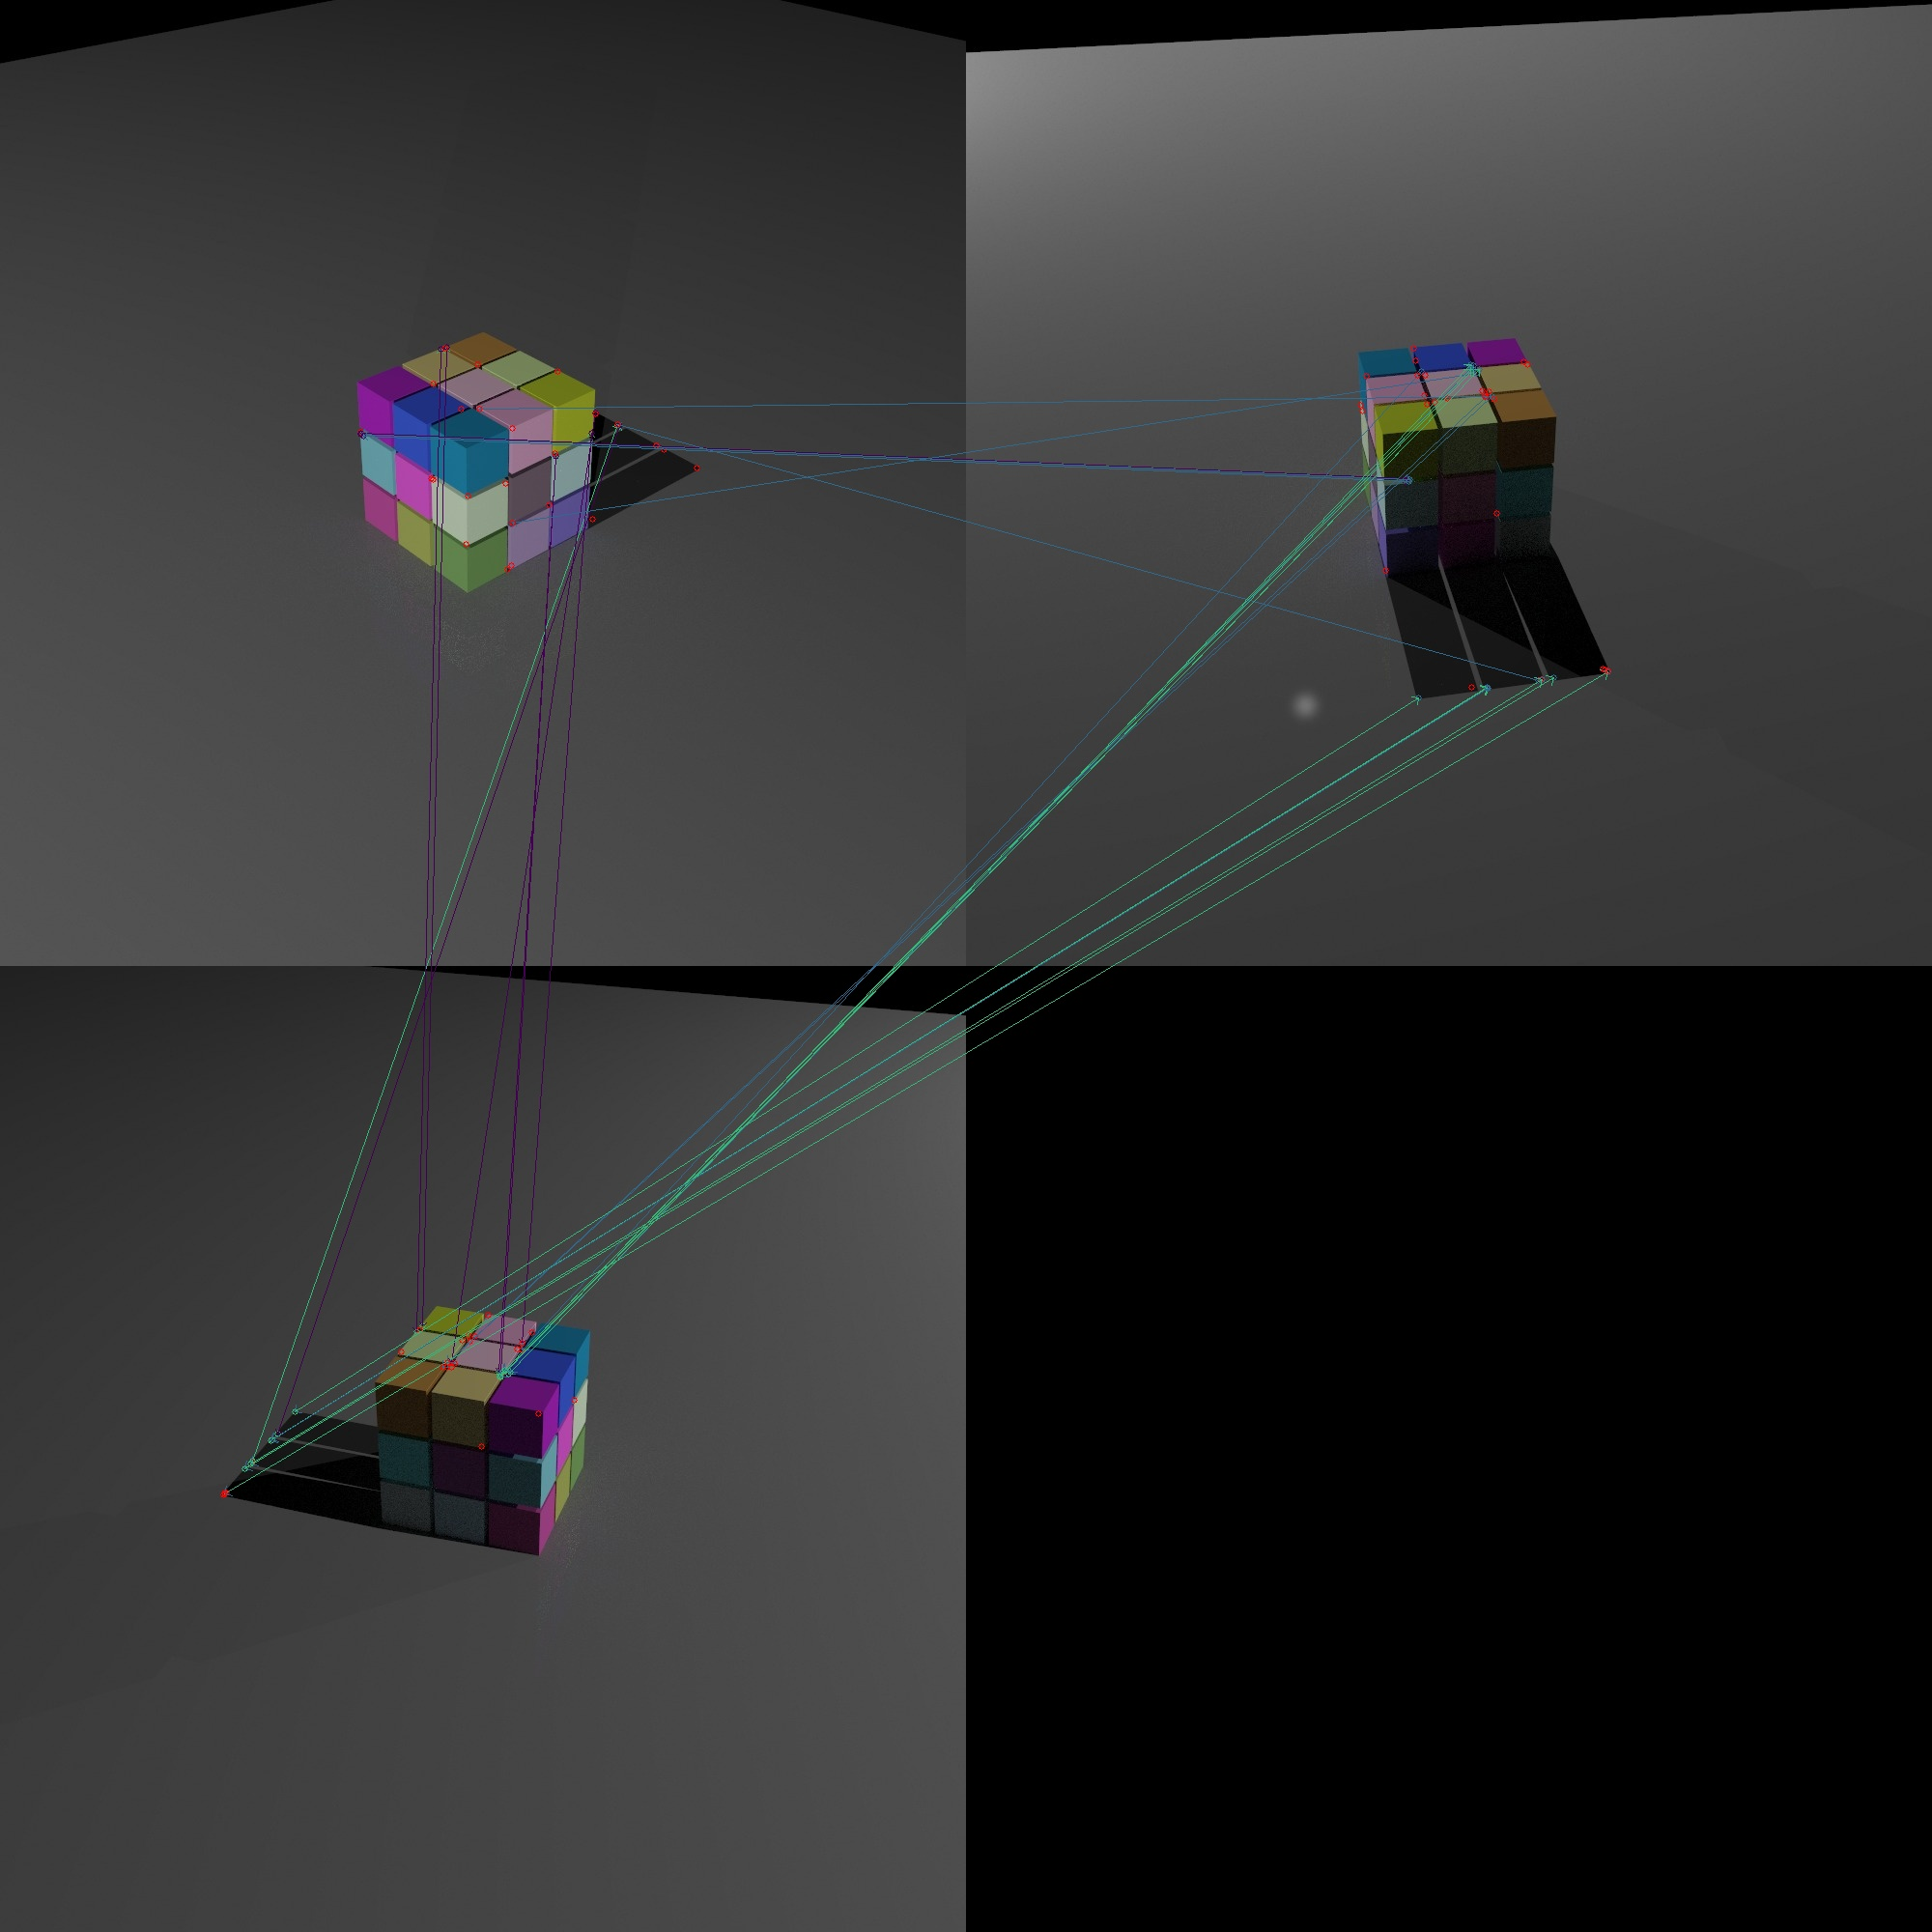
\includegraphics[width=0.3\textwidth]{img/filtered_image_graph.jpg}
  \end{figure}

\end{frame}


\begin{frame}{Bundle Adjustment}
  Using the image tracks, the final step of the problem is creating and solving
  a non-linear system of equations on the form:
  % 
  \begin{equation*}
    \mathbf{x}_{j} = f(\mathbf{X}_{i})
  \end{equation*}
  % 
  Where $\mathbf{X}_{i}$ represents a 3D point in the scene and $\mathbf{x}_{j}$
  is the projected image point of $\mathbf{X_{i}}$ from camera $j$. Here,
  $f(\cdot)$ represents function that transforms the 3D point to the image point.
\end{frame}

\begin{frame}{Ceres Functions}
  Using Ceres, the function $f(\cdot)$ can be written as a plain \texttt{C++}
  function and be automatically differentiated for computing e.g., the Jacobian
  matrix necessary for the optimization process.

  \lstinputlisting[style={google-c++},basicstyle={\tiny}]{lst/ceres.cpp}

\end{frame}


\begin{frame}{Results}

  Below are some examples of the recovered 3D structure from our procedures. Red
  points are scene points, green points correspond to cameras.

  \begin{columns}
    \begin{column}{0.5\columnwidth}
      \begin{figure}
        \centering
        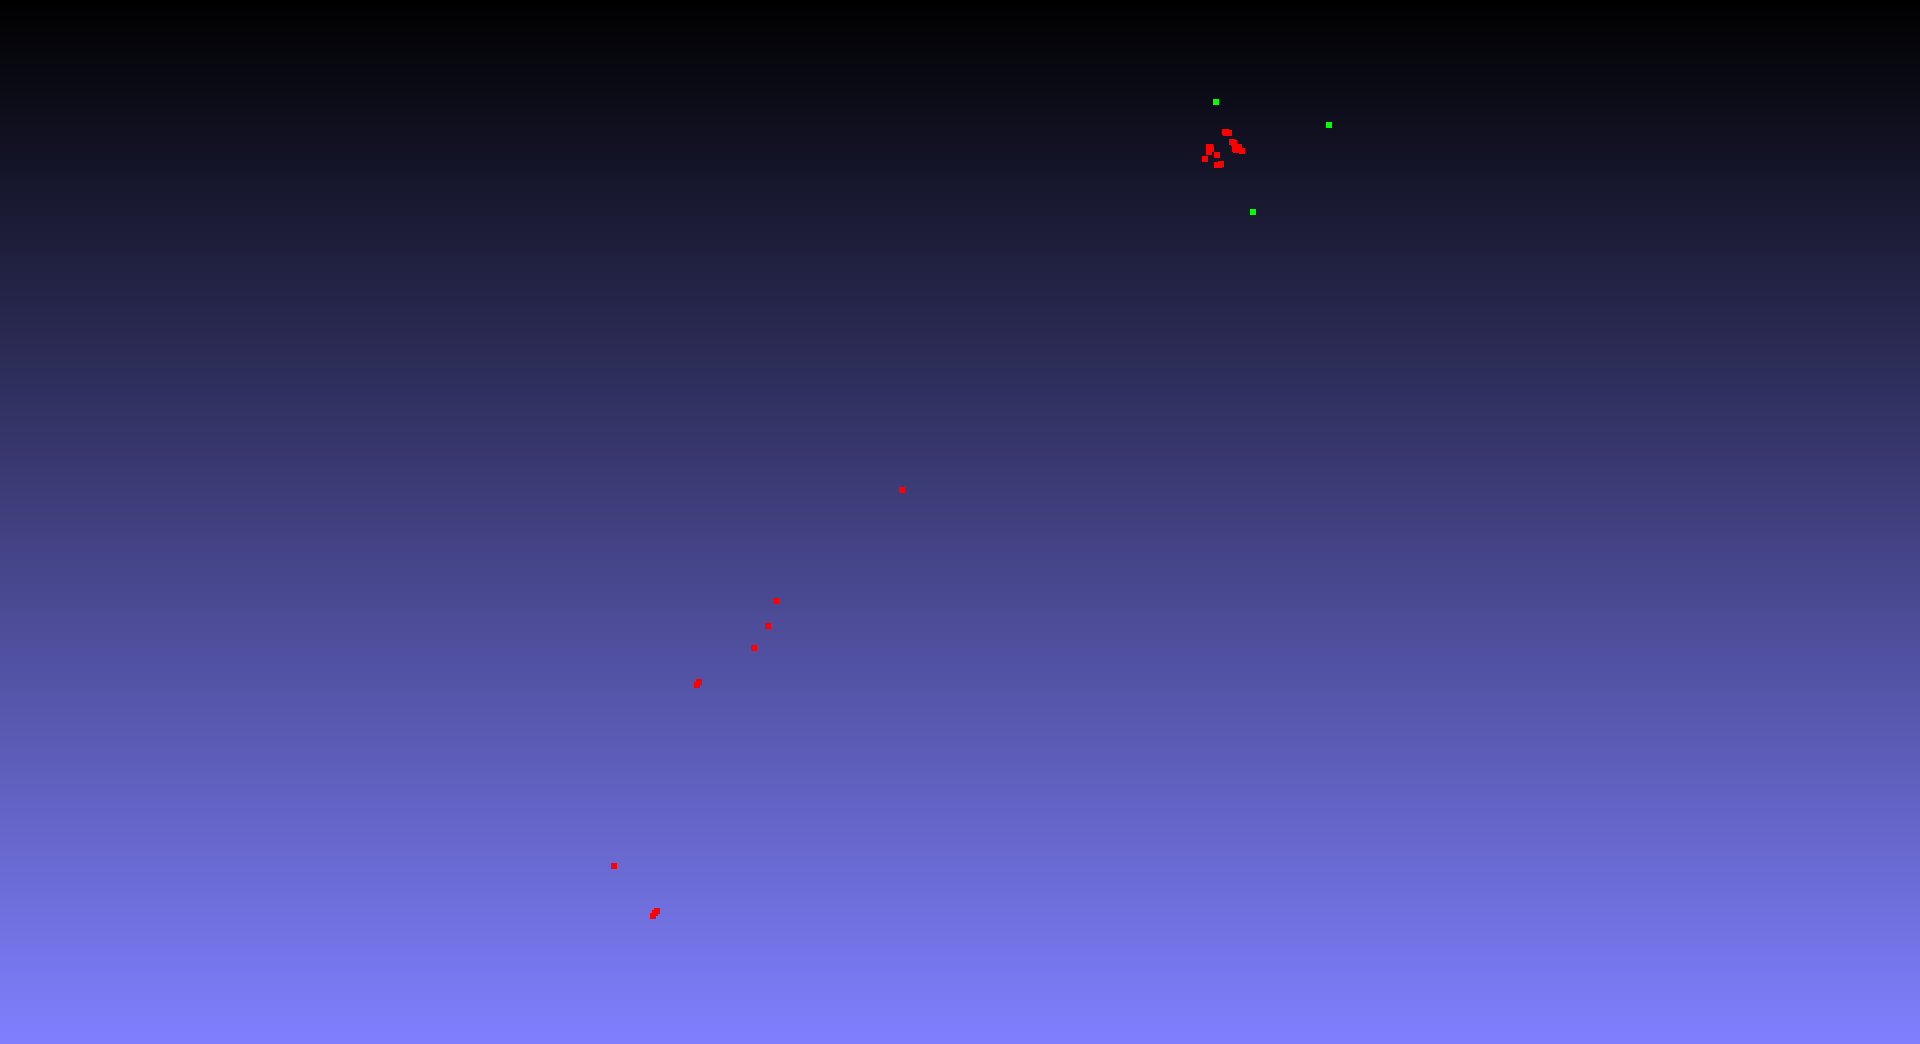
\includegraphics[width=1.0\textwidth]{img/sfm_all}
      \end{figure}
    \end{column}
    \begin{column}{0.5\columnwidth}
      \begin{figure}
        \centering
        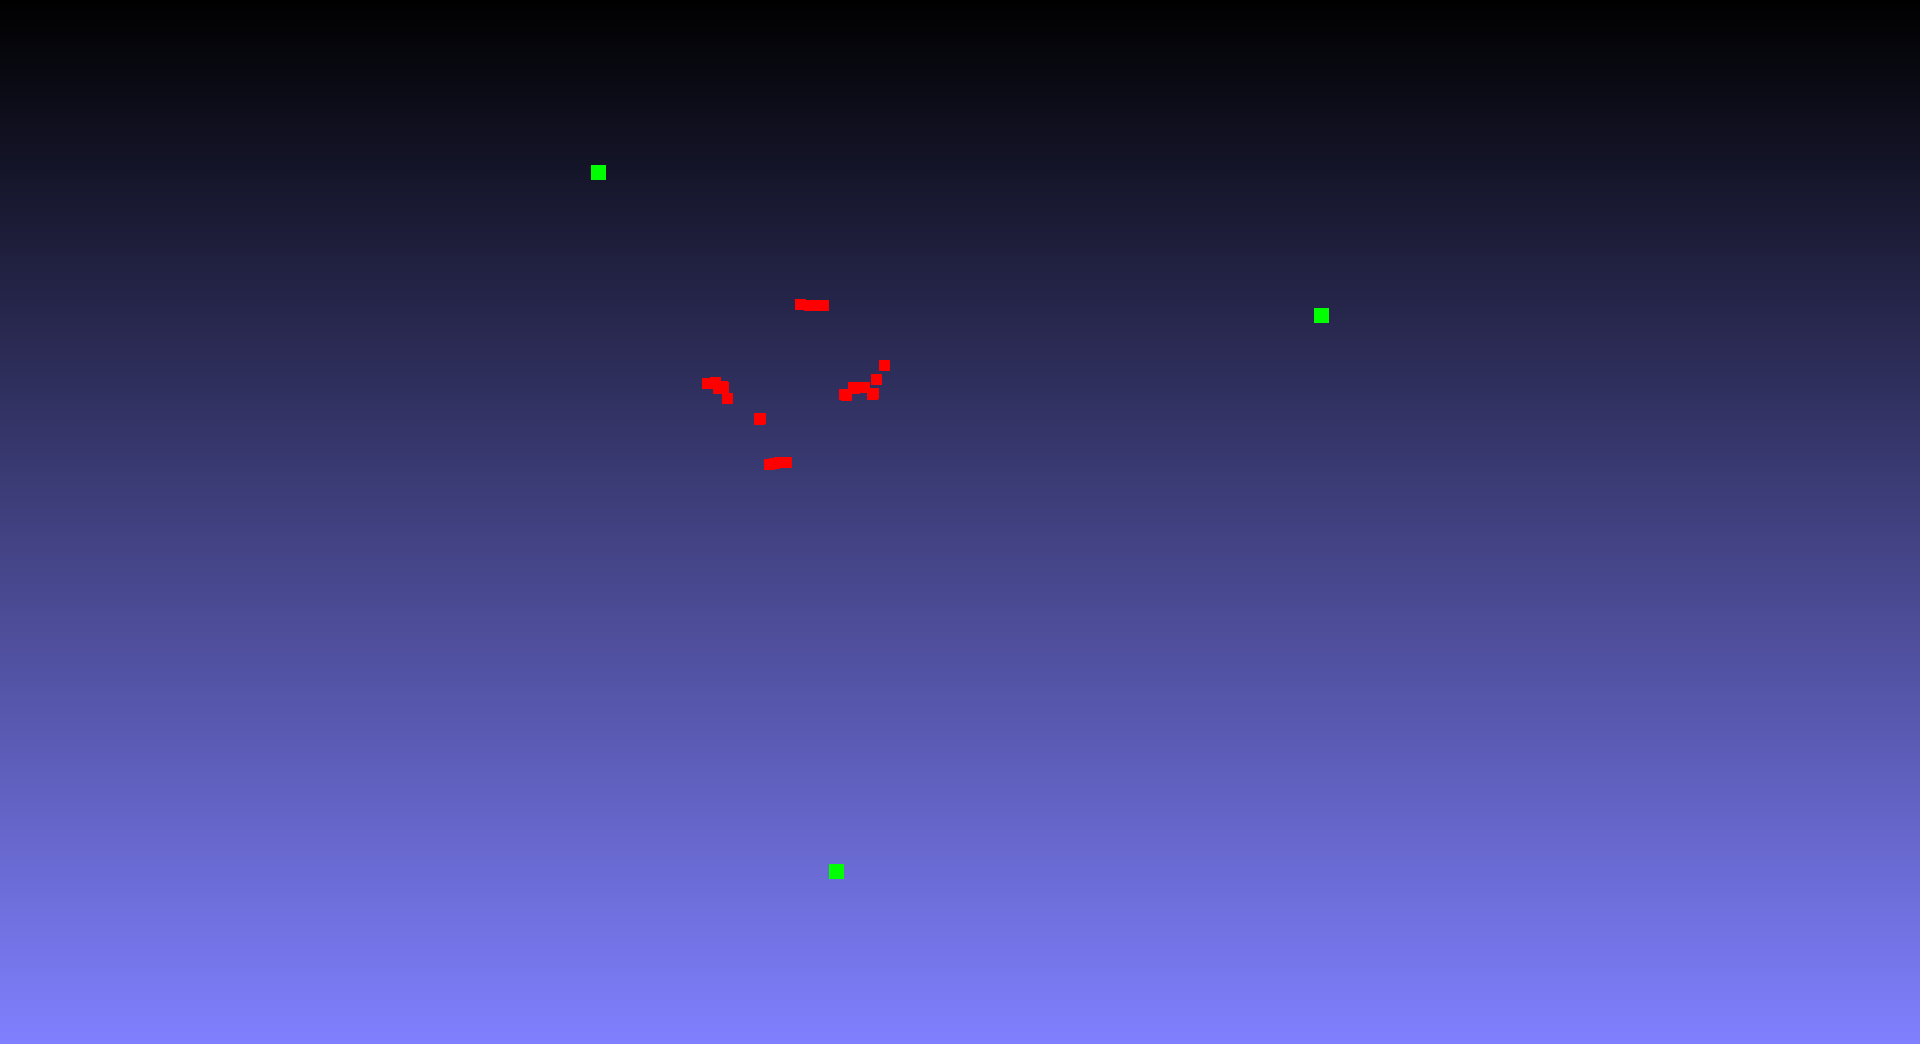
\includegraphics[width=1.0\textwidth]{img/sfm_filtered}
      \end{figure}
    \end{column}
  \end{columns}

  \vspace{0.2cm}
  Note that the right image have been manually filtered to remove outliers.

\end{frame}

\begin{frame}{Future Work}

  This project fell a bit short in respect to the amount of work necessary to
  complete a full system. To that end, a number of avenues for future work was
  identified:

  \begin{description}
  \item[Image matching] Robustly identify when one or more cameras are
    not looking in the same direction.
  \item[Graph/Network filtering] Since the problem can be translated into a
    graph, there are a wide number of graph based algorithms that could be
    applied to simplify the filtering process.
  \item[Parallelization] While our procedure have several synchronization
    points, there are many opportunities for parallelization or acceleration on
    GPUs.
  \end{description}

\end{frame}

\bgroup
\setbeamertemplate{background}{}
\setbeamercolor{background canvas}{bg=black}
% \setbeamertemplate{navigation symbols}{}
\begin{frame}[t,plain]{}{}
  \begin{center}
    {\tiny \textcolor{white}{The End}}
  \end{center}
\end{frame}
\egroup

\end{document}
